 \documentclass[CMPE]{KGCOEReport}

\usepackage{float}
\usepackage{graphicx}
\usepackage{amsmath}
\usepackage{kmap}
\newcommand{\classCode}{CMPE 160}  
\newcommand{\name}{Christopher Larson}
\newcommand{\LabSectionNum}{L3}
\newcommand{\LabInstructor}{Mr.\ Dominguez}	
\newcommand{\TAs}{Andrew Ramsey \\ Matthew Millar \\ Madeline Mooney}
\newcommand{\LectureSectionNum}{01}
\newcommand{\LectureInstructor}{Professor Beato}
\newcommand{\exerciseNumber}{06}
\newcommand{\exerciseDescription}{Binary Addition and Subtraction Circuits }
\newcommand{\dateDone}{21 February 2018}
\newcommand{\dateSubmitted}{28 February 2018}

\begin{document}
\maketitle

\section*{Abstract}
The objective of this exercise was to desgin, and implement binary artihmetic circuits, such as a one-bit full adder and a four-bit full adder/subtractor. The full adder was designed and constructed using basic logic gates, and the four-bit full adder/subtractor was built using a four-bit full adder chip. Full-adders perform addition between two binary numbers and accounts for values carried in as well as out. For a one-bit adder there are three inputs, A, B and Carry-In and two outputs, the Sum and the Carryout. The four-bit adder takes in nine inputs and returns five outputs, and uses twos-complement to represent negative numbers. The one-bit adder was expressed as a boolean expression and simplified using a Karnaugh map, which was used to to build a schematic diagram of the circuit. The schematic was used to simulate the waveforms of the one-bit adder to confirm the correct of the circuit by comparing it against a test bench, the waveforms and design of the circuit were shown to be correct. Once the design was found to be correct the schematic was transferred onto a breadboard and tested for correctedness, which it was found to be. A four-bit adder/subtractor was also designed and transferred onto a breadboard, which was tested for correctedness by comparing the results to hand-computed results. The four-bit adder/subtractor was found to be correctly designed as the tested results matched the expected results.

\section*{Design Mathodology}
The boolean expression used to create the sum of products expressions was $Sum = \Sigma_{ABCin}(1,2,4,7)$ and $Carryout = \Sigma_{ABCin}(3,5,6,7)$ . The Karnaugh map respresentations of the expressions are shown in Figure 1 for the Sum and Figure 2 for the CarryOut. 

\begin{figure}[H]
	\centering
	\begin{Karnaugh3Var}[A][B][Cin]
		\contingut{0,1,1,0,1,0,0,1}
		\implicant[2pt]{1}{1}{blue}
		\implicant[2pt]{2}{2}{blue}
		\implicant[2pt]{4}{4}{blue}
		\implicant[2pt]{7}{7}{blue}
		\end{Karnaugh3Var}
		\caption{K-map of Sum}
		\label{fig:Figure 1}
\end{figure}

The equation given from the K-map in Figure 1 is shown in Equation 1. This expression was further simplified by changed the AND and OR gates to XOR, shown in Equation 2.

\begin{equation} Sum = \overline{A}\,\overline{B} Cin + X\overline{Y}\,\overline{Cin} + \overline{X}Y\overline{Cin} + XYCin \end{equation}
\begin{equation} Sum = (X \oplus Y) \oplus Cin \end{equation}

Figure 2 shows the Carryout Karnaugh map.

\begin{figure}[H]
	\centering
	\begin{Karnaugh3Var}[A][B][Cin]
		\contingut{0,0,0,1,0,1,1,1}
		\implicant[2pt]{3}{7}{blue}
		\implicant[2pt]{5}{7}{blue}
		\implicant[2pt]{7}{6}{blue}
		\end{Karnaugh3Var}
		\caption{K-map of Cout}
		\label{fig: Figure 2}
\end{figure}

The equation given from the K-map in Figure 2 is shown in Equation 3. This is the sum of products equation with the minimal amount of terms.

\begin{equation} Carryout = XY + \overline{X}YCin + X\overline{Y}Cin \end{equation}

Using Equation 2, a circuit diagram was drawn to represent both the Sum and Carryout expression. This circuit diagram is shown in Figure 3, both expressios ise the same inputs but go to different outputs represent as Sum and Cout.

\begin{figure}[H]
	\centering
	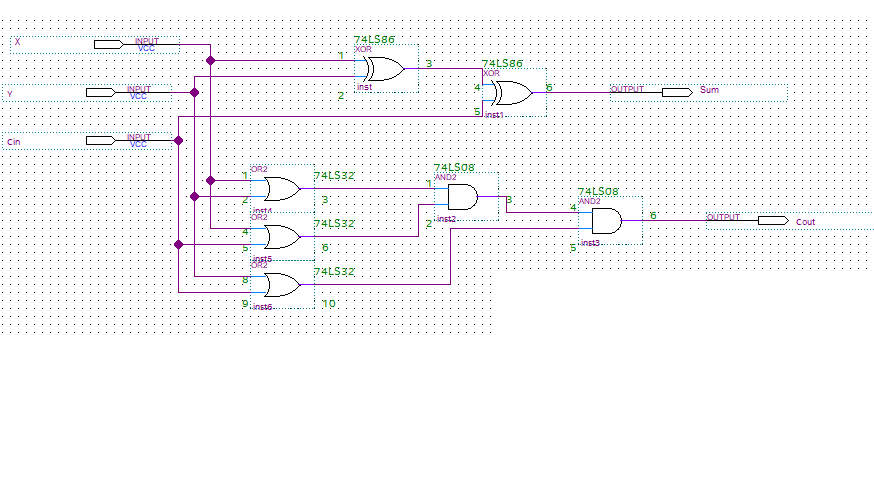
\includegraphics[width=1.0\textwidth]{QuartusL6}
	\caption{The schematic diagram of the Sum and Cout expressions}	
	\label{fig: Figure 3}
\end{figure}

A schematic diagram was also designed for the four-bit adder/subtractor shown in Figure 4. The way the adder/subtractor knows whether to add or subtract is by using a control line represented in Figure 4 as Co, which told the chip whether to add or subtract. The four-bit numbers were also represented in twos-complement,where if the number was negative the binary 1s and 0s would be flipped and one would be added to the number, this allowed for negatives to be added and subtracted.

\begin{figure}[H]
	\centering
	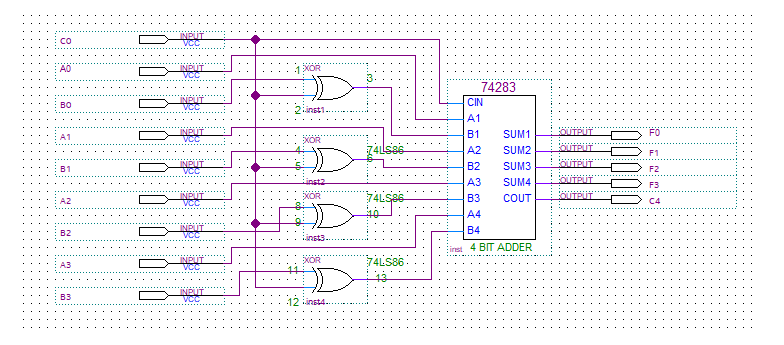
\includegraphics[width=1.0\textwidth]{QuartusL6PT2}
	\caption{The schematic diagram of the four-bit adder/subtractor}
	\label{fig: Figure 4}
\end{figure} 

The circuit diagram in Figure 3 was used to simulate the waveform of the equation and compared to a test bench to confirm the correctness of the circuit. The schematic in Figure 3  and Figure 4 were also used to implement the one-bit full adder and four-bit adder/subtractor circuit on the breadboard, to show the correctness of the schematic, and the four-bit adder/subtractor results table.

\section*{Results}

The waveform in Figure 5 matched the waveform in the test bench exactly and shows the circuit diagram was correct. 

\begin{figure}[H]
	\flushleft
	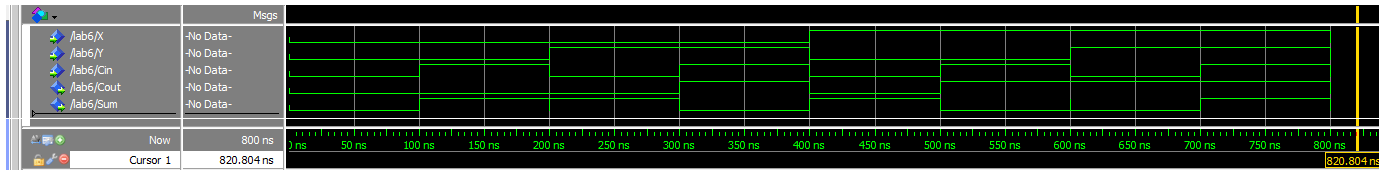
\includegraphics[width=1.0\textwidth]{ModelSimL6}
	\caption{The ModelSim representation of Sum and Carryout}
	\label{fig: Figure 5}
\end{figure}

A table was also given to test the accuracy of the four-bit full adder/subtractor, this tested the subtraction and addition functions by giving two four-bit numbers. Some of the numbers that were given were unable to be represented in the five bits of output that the four-bit full adder/subtractor has and therefore shows the limited capability of the four-bits. Table 1 shows the expected results in decimal and the results that actually occurred in binary.

\begin{table}[H]
	\centering
	\caption{Four-bit addition and subtraction}
	\label{tab: Table 1}
	\begin{tabular}{|c|c||c||c||c|}
		\hline
		A3 A2 A1 A0 & B3 B2 B1 B0 & C4 & F3 F2 F1 F0 & A + B = F\\ \hline
		S7 S6 S5 S4 & S3 S2 S1 S0 & L4 & L3 L2 L1 L0 & (Decimal)\\ \hline
		0011 & 0100 & 0 & 0111 & (3) + (4) = 7\\ \hline
		1010 & 0101 & 0 & 1111 & (-6) + (5) = -1\\ \hline
		1010 & 0011 & 0 & 1101 & (-6) + (3) = -3\\ \hline
		1111 & 0110 & 1 & 0101 & (-1) + (6) = 5\\ \hline
		1111 & 1111 & 1 & 1110 & (-1) + (-1) = -2\\ \hline
		A3 A2 A1 A0 & B3 B2 B1 B0 & C4 & F3 F2 F1 F0 & A - B = F\\ \hline
		S7 S6 S5 S4 & S3 S2 S1 S0 & L4 & L3 L2 L1 L0 & (Decimal)\\ \hline
		0111 & 0011 & 1 & 0100 & (7) - (3) = 4\\ \hline
		1010 & 0011 & 1 & 0111 & (-6) - (3) = 7\\ \hline
		1111 & 0110 & 1 & 1001 & (-1) - (6) = -7\\ \hline
		1111 & 1111 & 1 & 0000 & (-1) - (-1) = 0\\ \hline
		0101 & 1010 & 0 & 1011 & (5) - (-6) = -5\\ \hline
		\hline
	\end{tabular}
\end{table}	

\section*{Conclusion}

The use of K-maps and boolean algebra to create and design binary arithmetic circuits allows for the most efficient version of the circuit to be made. It is important to confirm the simplifed equations are equal to expected equation using Modelsim to compare the waveforms of the schematic, as well as use a results table to confirm the correctness of the four-bit full adder/subtractor. The exercise proved successful for both the one-bit full adder and four-bit full adder/subtractor.

\section*{Questions}
1.
\begin{figure}[H]
	\centering
	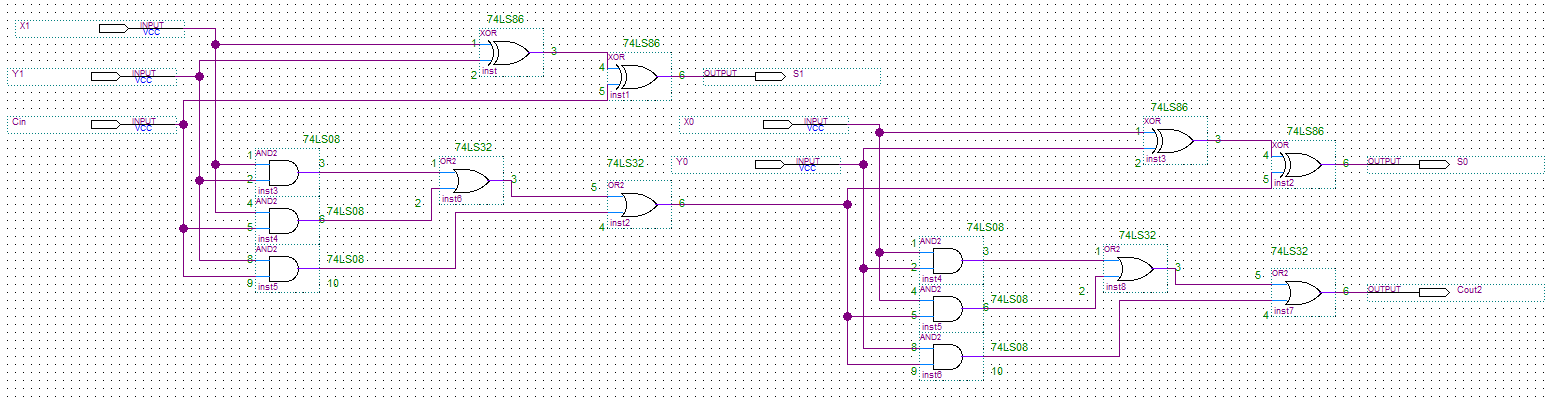
\includegraphics[width=1.0\textwidth]{QuartusL6Q1}
	\caption{Diagram of a two-bit carry-ripple adder}
	\label{fig: Figure 6}
\end{figure}\break

2.
The overflow can be detected if the most significant bit and the carryout of the most significant bit are XORed together as shown in Equation 4.
\begin{equation} C2 \oplus C3 \end{equation}\break

3. The four bit adder/subtractor produces incorrect two's complement results when there is an overflow because it does not have any way of dealing with numbers outside the range of 7 to -8.\\

4. No the correct answer would still not be found, the equation (-1) + (6),(1111 + 0110) would return 10101 which is equal to (-11) not (5), which is the correct answer.\break

5.
\begin{figure}[H]
	\centering
	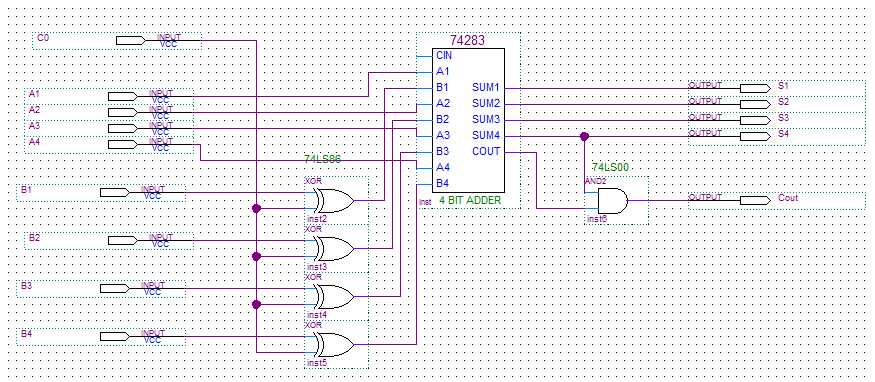
\includegraphics[width=1.0\textwidth]{QuartusL6Q2}
	\caption{Diagram of a 4-bit adder/subtractor}
	\label{fig: Figure 7}
\end{figure}\break
\end{document} 